\chapter{Étude du nœud A}
Dans cette partie, nous étudierons un premier bloc du réseau. Nous calculerons les courbes d'arrivé du noeud et la courbe de service pour comprendre sa courbe de sortie et ainsi mesuré sa porter sur le reste du réseau.

Les tracés de l'ensemble des courbes a été obtenu par l'interpréteur en ligne \emph{http://realtimeatwork.com/minplus-playground}, il s'agit d'un interpréteur qui permet entre autre le tracé de courbes affines mais aussi le calcul en algèbre (min,+). 

Nous avons décidé de d'utiliser et de fixer les unités sur lesquelles nous baserons nos courbes. Nous avons choisi de travailler en \textbf{octets} (axe des ordonnées) et le temps (axe des abscisse) sera en \textbf{millisecondes}. Nous verrons en synthèse à ce rapport si nos choix pour ces unités étaient judicieux. \label{fixUnity}

\section{Courbes d'arrivée $\alpha$} 
Pour déterminer la courbe d'arrivée, nous allons tout d'abord analyser les données que nous pouvons receuillir sur le bloc A. Nous relevons deux flux d'entrée $v1$ et $v2$. Pour connaitre la courbe d'arrivée $\alpha^A$, nous devons tracer les deux courbes d'entrée des deux flux entrants, courbes que nous affichons en figure (\ref{fig:CA_1_2})

\begin{figure}[!ht]
\centering
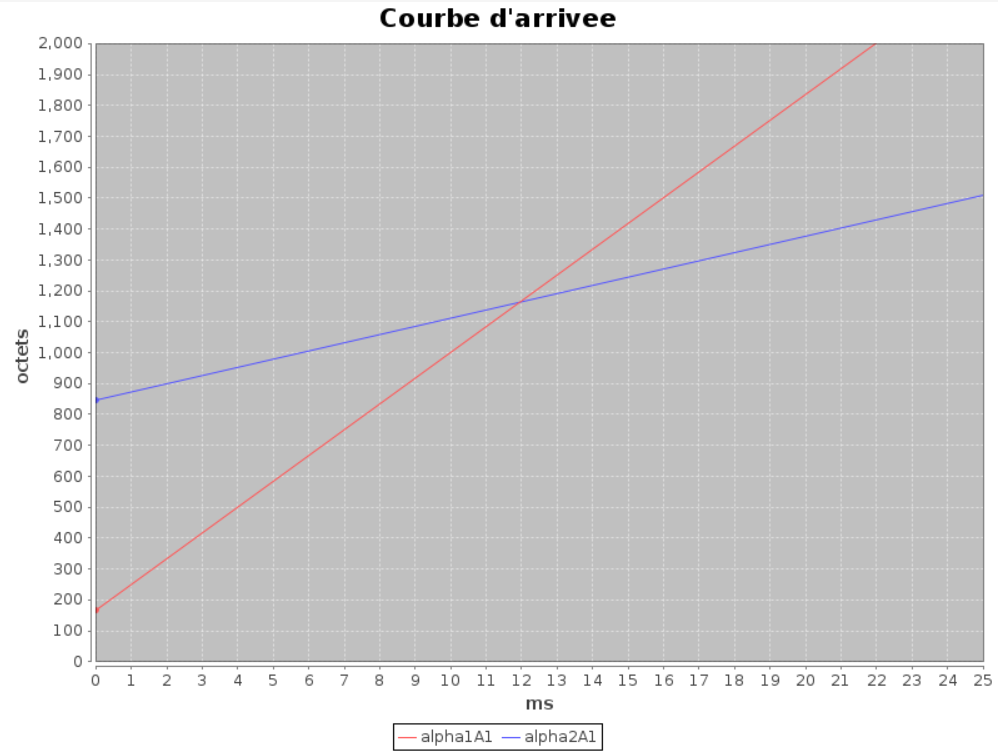
\includegraphics[width = .6\textwidth]{./I/images/alpha_1_2.png}
\caption{\label{fig:CA_1_2}Courbe d'arrivée $\alpha$ du flux $v1$ (rouge) et du flux $v_2$ (bleu)}
\end{figure} 

Ces courbes ont été obtenu à l'aide des informations sur les $BAG$ et les $s_{max}$ de $v1$ et $v2$. Pour obtenir des données correspondantes aux unités choisis en \ref{fixUnity}, nous devons utiliser la relation suivantes qui lie la taille maximale d'une trame $L_j^{max}$ et la charge utile maximale $s_j^{max}$ d'un \emph{Virtual Link}(VL) $j$ :
\begin{align}\label{eqn:maxTrame}
L_j^{max} = max(s_j^{max},17)+47
\end{align}
Nous observons donc avec cette équation que la taille maximale d'une trame est strictement supérieure à $50$. A l'aide de cette équation, nous sommes capable d'établir la pente $a_j$ de la courbe des données maximales ainsi que son offset $b_j$ de décalage qui peuvent arrivées dans $A$ avec \begin{align}\label{eqn:penteOffset}
 &a_j = \frac{L_j^{max}}{BAG_j}\\
 &b_j = L_j^{max}
\end{align}

Dans notre cas, nous obtenons l'application numérique suivante : 
\begin{align*}
&a_1 = \frac{L_1^{max}}{BAG_1} = \frac{ max(s_j^{max},17)+47}{BAG_1} = \frac{167}{2} = 83.5\\
&b_1 =  max(s_j^{max},17)+47 = 167
\end{align*}
Avec l'interpréteur, nous pouvons obtenir la courbe affine avec la commande : \begin{verbatim}
alpha1A1 := affine(83.5, 167) //echelle octets/ms
\end{verbatim}

De même pour le flux $v2$,nous obtenons comme application numérique : \begin{align*}
&a_2 = 26.46\\
&b_2 = 847
\end{align*}
La courbe obtenu est de la forme sceau percé, nous avons une quantité maximale émise instantanément par le bloc $A$ et un débit moyen maximal.
\section{Courbe de service $\beta$}
Nous allons maintenant établir la courbe de service disponible par le nœud A. Cette fonction du port desortie de $A$ est établit en fonction de la latence technologique $\mu$ déterminé et du débit du port de sortie. Notre étude est calibré selon lesuniés défini en\ref{fixUnity}, il est donc important de respecter ces conditions dès maintenant pour éviter tout problème fuur d'unité. Nous relevons :\begin{align}\label{eqn:portSortie}
debit &= 100Mb/s = 12500\ Octets/ms\\
\mu &= 16\mu s = 0.016 ms
\end{align}

Pour établir cette fonction sur \emph{Network Calculus}, nous avons choisi d'établir une fonction affine qui admet comme pente le débit du port de sortie mais qui subit un décalage, i.e un \emph{delay} dans l'interpréteur, pour modéliser la latence technologique. La courbe en \ref{fig:serviceA} est obtenu avec la ligne de commande :
\begin{verbatim}
betaA := affine(12500,0) * delay(0.016) 
\end{verbatim}
\begin{figure}[!ht]
\centering
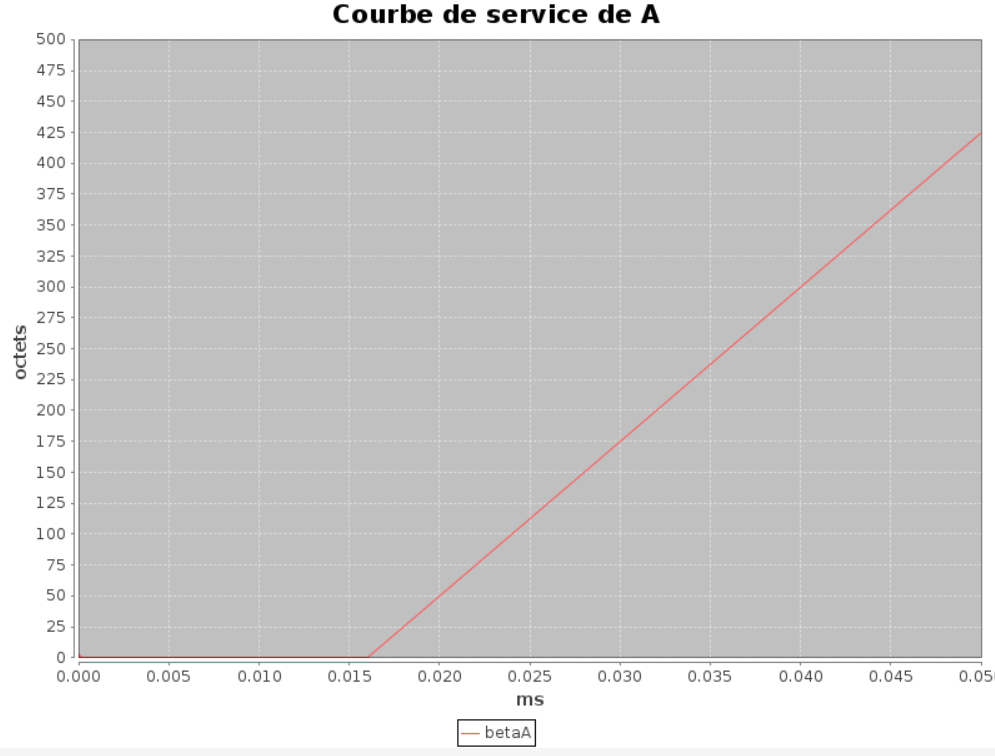
\includegraphics[width = .5\textwidth]{./I/images/beta_A.png}
\caption{\label{fig:serviceA}Courbe de service du nœud A}
\end{figure} 

Cette courbe est du type latence-taux, car notre modèle admet une latence technologique et dispose d'un débit de sortie. Pour résumé, le modèle du nœud $A$ reçoit des données dans une courbe d'arrivé de type seau percé pour les traiter avec une courbe de service du type latence-tau. Selon nos estimations, le nœud va donc lisser le débit des flux $v1$ et $v2$.

\section{Courbe d'arrivée du nœud A}
Nous nous intéressons maintenant au cumul des flux dans l'entrée du nœud $A$. Pour cela, nous allons utiliser le résultat expliqué en pendant les travaux dirigés qui expriment : 
\begin{equation}
\alpha^A = \alpha_1^A + \alpha_2^A
\end{equation}
soit la somme des pentes $r_i$ et des $L_i^{max}$ de $\alpha_1^A$ et $\alpha_2^A$. Nous obtenons par le calcul une fonction affine décrit dans l'équation  que nous comparons avec les courbes $\alpha_1^A$ et $\alpha_2^A$ dans la figure \ref{fig:arriveA}.
\begin{align}\label{eqn:arriveA}
&\alpha^A = \gamma_{r,b} \text{ avec $r$ la pente et $b$ les tailles maximales de la trame $L_i$}\\
&r = r_1 + r_2 = a_1 + a_2\text{ et } \\
&b = b_1 + b_2 = b_1 + b_2\\
\end{align}
\begin{figure}[!ht]
\centering
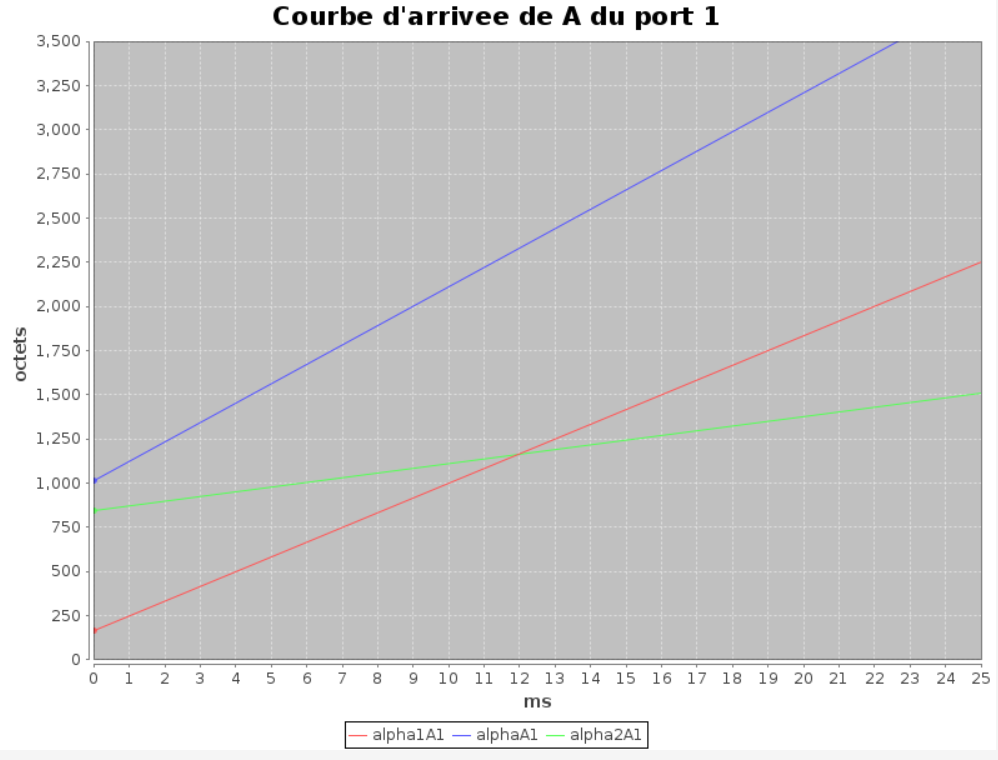
\includegraphics[width = .6\textwidth]{./I/images/arrive_general.png}
\caption{\label{fig:arriveA}Courbe de d'arrivé du nœud A}
\end{figure} 

\section{Délai et backlog pire cas}
Le délai pire cas et le backlog permettent de se concentrer sur l'étude des temps de traversé du système. Nous en aurons besoin dans le suite de ce rapport, c'est pourquoi nous commençons l'étude dans cette partie.

Pour déterminer ce temps et cette quantité de donnée, nous utilisons un résultat donné en cours qui explique les relations suivantes : le délai pire cas est la plus grande différence horizontale entre la courbe d'arrivé et la courbe de service d'un nœud noté \emph{hDev}. Respectivement, le backlog pire cas est la plus grande différence verticale entre les deux courbes noté \emph{vDev}. 

Nous obtenons ainsi un délai et une quantité qui représentent les pire cas possibles de traitement du nœud. Avec l'interpréteur de commande, nous pouvons calculer ces deux informations et nous obtenons : \begin{align}\label{eqn:delai-backlog}
&hDev(\alpha^{A1},\beta^A) = 2.36 ms\\
&vDev(\alpha^{A1},\beta^A) = 168.3\ octets
\end{align}
Nous ne connaissons pas les limites du système qui utilise ce réseau, nous ne pouvons donc pas établir de conclusions sur ces résultat. Nous pourrons les comparer une fois que les délai et backlog pire cas des autres nœud auront été calculé.

\section{Courbes d'arrivée des ports 1 et 2 de $B$}\label{sub:sortiesAs}
Avec la mise en tandem des flux $v1$ et $v2$, nous pouvons établir la courbe d'arrivé du bloc $B$ avec les courbes de sorties du bloc $A$. Nous disposons de l'équation qui permet de lié la courbe d'arrivé avec la courbe de sortie :
 \begin{equation}
\alpha_i^{B_i} = \alpha'^{A_i} = \alpha^{A_i} \varoslash \tau_i
\end{equation} avec $tau$ le délai pire cas du flux $i$ et $\alpha'^{A_i}$ la courbe de sortie du bloc $A$ correspondant au flux $i$. Nous avons déjà calculé le délai pire cas du flux $1$ mais pas le flux $2$. Avec le même raisonnement utilisé en \ref{eqn:delai-backlog}, nous avons :
\begin{equation}
\tau_2 = hDev(\alpha^{A2}, \beta^{A}) = 83.7ms
\end{equation}
Maintenant que nous disposons de toutes les ressources, nous pouvons calculer les courbes d'arrivé des flux $1$ et $2$ dans $B$ avec l'interpréteur : \begin{verbatim}
alpha1B1 := alpha1A1 / delay(HdevA1)
alpha2B2 := alpha2A2 / delay(HdevA2)
\end{verbatim}
Ces réslutats nous permetent d'afficher la figure suivante :
\begin{figure}[!ht]
\centering
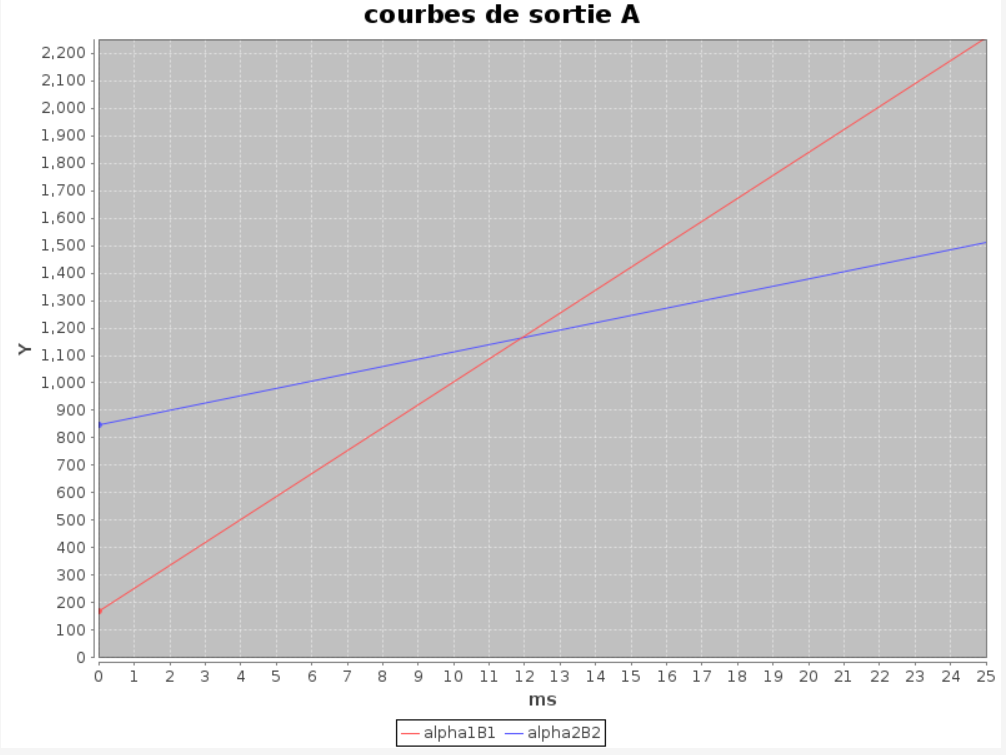
\includegraphics[width = .6\textwidth]{./I/images/sortiesA.png}
\caption{\label{fig:sortieA}Courbes de sortie du nœud A}
\end{figure} 
